\section{Desarrollo}

\parencite{molina2013unifying}

\subsection{Descripción del caso práctico}

El estudio presentado propone un controlador difuso unificado para mejorar la gestión de la calidad del ambiente interior (IEQ). Este enfoque busca superar las limitaciones de los sistemas tradicionales de control HVAC, que a menudo son incapaces de manejar de manera eficiente múltiples variables y criterios interrelacionados. 

El caso práctico analizado en la publicación consiste en aplicar el controlador difuso propuesto a una habitación piloto equipada con sensores de temperatura, humedad y calidad del aire. 

\subsection{Diseño del controlador difuso}

La propuesta incluye un controlador basado en lógica difusa, recomendado especialmente en aplicaciones donde el modelo matemático exacto del sistema no es conocido, pero su comportamiento puede ser descrito a partir de la experiencia. Este tipo de controlador mejora la flexibilidad ajustándose a los requisitos de confort y puede manejar situaciones críticas de manera más confiable, gracias a reglas basadas en el conocimiento experto.

\subsubsection{Entradas y salidas}

El sistema utiliza cinco sensores:

\begin{enumerate}
	\item Temperatura interna ($S_{temp_{indoor}}$)
	\item Temperatura externa ($S_{temp_{outdoor}}$)
	\item Humedad relativa ($S_{RH}$)
	\item Concentración de CO2 ($S_{CO_2}$)
	\item Nivel de iluminación ($S_{light}$)
\end{enumerate}

Las salidas son cuatro, que se corresponden a tres actuadores:
\begin{enumerate}
	\item Programa del aire acondicionado ($A_{Air}$): caliente, frío, seco.
	\item Nivel de temperatura ($A_{temp_{level}}$): bajar, mantener, subir.
	\item Nivel de iluminación ($A_{light}$): bajo, medio y alto.
	\item Nivel del humedad ($A_{h_{level}}$): apagado, bajo, estándar, alto, continuo.
\end{enumerate}

Estos actuadores regulan el confort del ambiente interior al influir en el sistema HVAC. Las decisiones sobre estas salidas se toman con base en las lecturas de los cinco sensores y se ajustan dinámicamente según las reglas difusas definidas en el sistema

\subsubsection{Funcionamiento del controlador}

El FLC se basa en un motor de inferencia, que procesa las entradas tras la fuzzificación y genera salidas mediante un proceso de defuzzificación. Esto permite ajustar el sistema para lograr el confort del usuario. REVISAR.

\begin{figure}[H]
	\centering
	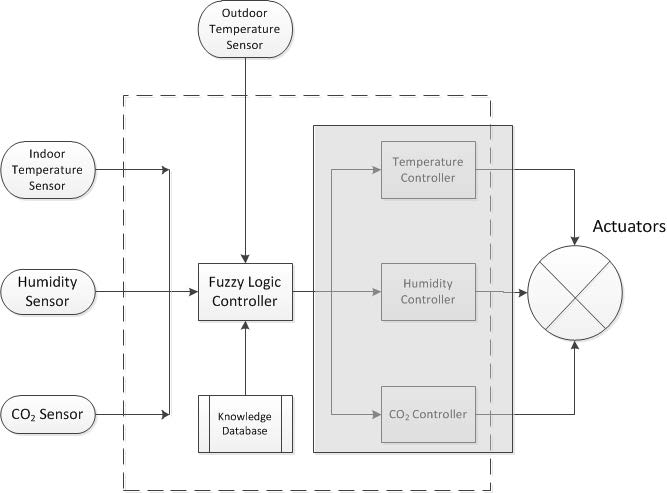
\includegraphics[width=0.85\textwidth]{imgs/arquitectura-FLC.JPG}
	\caption{Arquitectura PID y controlador fuzzy}
	\label{fig:arquitectura-FLC}
\end{figure}

La \autoref{fig:arquitectura-FLC} muestra la arquitectura del FLC, diseñado para regular diferentes variables ambientales mediante un conjunto de sensores y actuadores. Los sensores monitorean parámetros clave, como la temperatura interna y externa, la humedad y la concentración de CO2. Estas lecturas se envían al controlador difuso, que analiza los datos en combinación con una base de conocimiento. Esta base de conocimiento contiene reglas y relaciones definidas por expertos que permiten al sistema tomar decisiones informadas.

El controlador difuso procesa las entradas y determina las acciones necesarias para mantener las condiciones óptimas dentro del entorno. Las decisiones se transmiten a una serie de controladores específicos para cada variable, como el controlador de temperatura, el de humedad y el de CO2. Finalmente, estos controladores ajustan los actuadores correspondientes para implementar las acciones recomendadas. De esta manera, el sistema asegura un ambiente confortable y eficiente, gestionando las interdependencias entre las distintas variables

\vspace{0.4cm}

La \textbf{base de conocimiento} del FLC incluye:
\begin{enumerate}
	\item \textbf{Funciones de membresía}: se utilizan funciones trapezoidales para describir las etiquetas lingüísticas (Bajo, Medio, Alto).
	\begin{figure}[H]
		\centering
		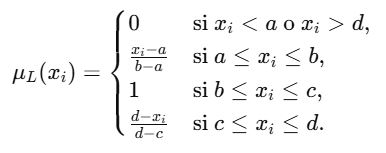
\includegraphics[width=0.55\textwidth]{imgs/function.JPG}
		\caption{Función de membresía}
		\label{fig:function}
	\end{figure}
	
	Se explican algunas variables de la \autoref{fig:function}: $L$ puede tomar el valor de Bajo, Medio y Alto; $a$ y $d$ son los puntos extremos de la función de membresía trapezoidal; $b$ y $c$, los puntos máximos de la función de membresía trapezoidal; y $x_i$ es el $i$-ésimo sensor.
	
	\begin{figure}[H]
		\centering
		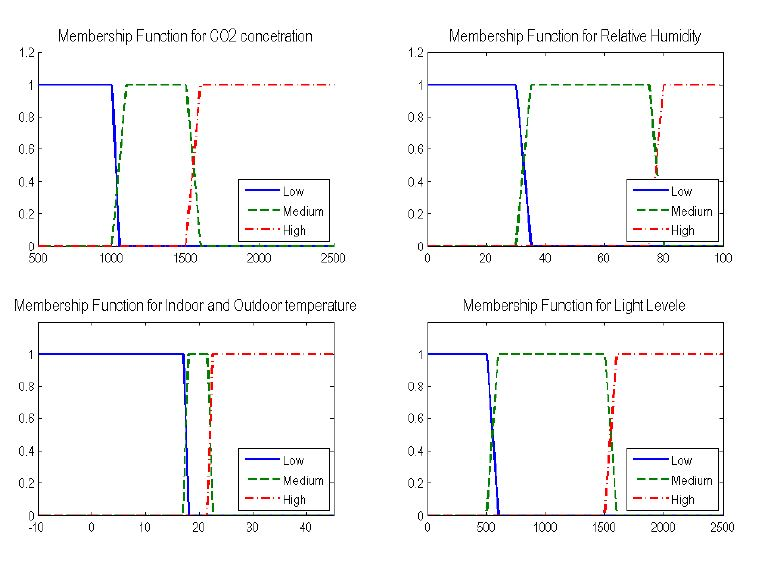
\includegraphics[width=0.8\textwidth]{imgs/membership-functions-input.JPG}
		\caption{Función de membresía de las variables de entrada}
		\label{fig:membership-functions-input}
	\end{figure}
	
	\begin{figure}[H]
		\centering
		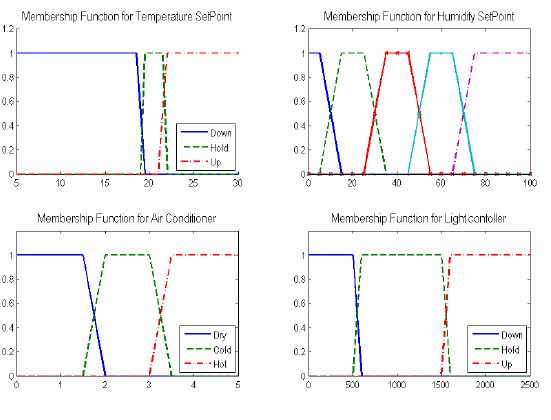
\includegraphics[width=0.8\textwidth]{imgs/membership-functions-output.JPG}
		\caption{Función de membresía de las variables de salida}
		\label{fig:membership-functions-output}
	\end{figure}
	
	\item \textbf{Reglas difusas}: conjunto de reglas IF-THEN derivadas del conocimiento experto. Ejemplos:
	\begin{itemize}
		\item Si la temperatura interna es Media y la externa es Alta, entonces mantener la temperatura y el humidificador en nivel estándar.
		\item Si la humedad es Baja y la temperatura interna es Baja, entonces el aire acondicionado debe estar en caliente, el humidificador en nivel Alto, y subir la temperatura.
	\end{itemize}
	
	Se han utilizado 17 reglas, que dan lugar a diversos escenarios al combinar las posibles entradas del sistema. Se muestra un subconjunto de las reglas en la \autoref{fig:set-of-rules}.
	
	\begin{figure}[H]
		\centering
		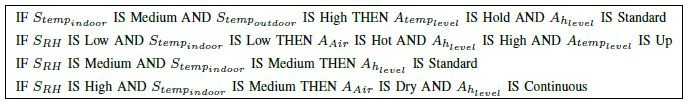
\includegraphics[width=0.9\textwidth]{imgs/set-of-rules.JPG}
		\caption{Conjunto de reglas}
		\label{fig:set-of-rules}
	\end{figure}
	
\end{enumerate}

El motor de inferencia aplica el \textbf{método Mamdani max-min} para combinar reglas y calcular las salidas. Este método evalúa el grado en que cada regla se cumple y combina las salidas difusas.

\begin{figure}[H]
	\centering
	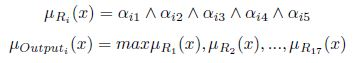
\includegraphics[width=0.55\textwidth]{imgs/mamdani.JPG}
	\caption{Método mamdani max-min}
	\label{fig:mamdani}
\end{figure}

En la \autoref{fig:mamdani}, $x$ son las mediciones de los sensores de entrada, $\alpha_i$ es el grado en que una entrada dada satisface la condición de la $i$-ésima regla ($R_i$), y $\mu_{output_i}$ es la agregación de los conjuntos difusos de salida de todas las reglas para $output_i$.

\subsection{Simulación y pruebas}

\subsubsection{Pruebas con el simulador}

\subsubsection{Pruebas experimentales}

\subsection{Resultados del estudio}
- resumen de resultados

Los resultados obtenidos del estudio indican que el controlador difuso logró mantener las condiciones ambientales dentro de los rangos de confort definidos, con una notable reducción en las fluctuaciones de temperatura y humedad. Durante el período de prueba, el controlador mostró un mejor desempeño que los sistemas reactivos, proporcionando un ambiente más estable y confortable para los ocupantes

- interpretación de los mismos

Estos hallazgos destacan la eficacia del controlador difuso para mejorar la gestión de la calidad ambiental interior. La capacidad del sistema para ajustarse dinámicamente a las condiciones cambiantes del entorno permitió no solo mejorar el confort, sino también optimizar el uso de energía. Esto subraya el potencial de la lógica difusa como una solución integral para sistemas HVAC avanzados en contextos de edificios inteligentes

